\documentclass{article} % For LaTeX2e
\usepackage{nips13submit_e,times}
\usepackage{hyperref}
\usepackage{url}
\usepackage{graphicx}
\usepackage{adjustbox}
\usepackage{subcaption}
\graphicspath{{images/}}
%\documentstyle[nips13submit_09,times,art10]{article} % For LaTeX 2.09

\nipsfinalcopy % Uncomment for camera-ready version

\begin{document}

\title{Reddit Comment Generator - Project Report}
\author{Braulio Chavez \\
  \texttt{braulioc@stanford.edu}}
\maketitle

\begin{abstract}
In this work I describe the implementation of a recurrent neural network
language model (RNN-LM) to solve the problem of automatic generation of logical
comments for a specific context. The RNN makes use of LSTM cells to help keep
long term data dependencies, improving the performance of the model. For
completeness I compared the training evaluation of the LSTM cell vs the GRU cell
under the same conditions. Then I discuss the reactions that the generated
comments got from the Reddit community and how to improve the model in order to give it
more context and understanding of sentences.  \end{abstract}

\section{Introduction}
Recurrent neural networks (RNN) have been used in a wide array of machine
learning problems. They are known to be a generative model which is a
particularly interesting property. Recently there have been various attemps to
increase the creativity of these models. These approaches are applied to
generate a varied ammount of media like images, music or poems.

In this project I make use of the generative properties of the RNN to try to
atomatize the generation of comments especific to a provided context. The
applications of this are many: FAQ answering, forum like discussion, chatbots
that help accomplish a task, gmail's autoreply feature.

The potential of this is huge, it can create be a whole new human computer
interaction paradigm on how users deal with technology. If implemented correctly
people won't even be able to discern a bot from a human on the other side of the
conversation (Turing test). This applies to any form of communication. Companies
wouldn't need to spend as many resources to generate a valuable product or
experience to their customers, think of customer service and internal processes,
even increase the usefulnes and intelligence of their current products.

The approach to solve this problem was to use already proved RNN language
models. I used the help of LSTMs to help alleviate the long term data dependecy
loss issue, this practice improved the performance of the model. In order to have
a baseline I also experimented with a GRU which in practical terms it is a
modified LSTM with different keep and forget functions and internal mechanisms
which I'll describe later. Once these two models were trained I evaluated them
with perplexity.

\section{Background/Related Work}
Previous approaches have been taken to solve this problem. This project is
highly influenced by the work \textit{Recurrent neural network based language
model} by Mikolov et al. 2010 and can be thought as a practical application of
the RNN language model with small variations. The main modification was the use
of LSTM cells on the model structure. Such cell was first proposed by Hochreiter
and Schmidhuber 1997 in the paper \textit{Long Short-Term Memory}

\section{Approach}
After some experimentation (described in the next section) with different
hyperparameter configurations, and by comparing the use of LSTM and GRU cells. I
arrived to the following language model used for comment generation. The model
is a stacked RNN with two hidden layer LSTM cells to help with the long term
data dependency loss problem. Each hidden layer has 200 nodes. You can see a
graphic representation in figure~\ref{fig:rnndiagram}.

\begin{figure}[h]
\centering
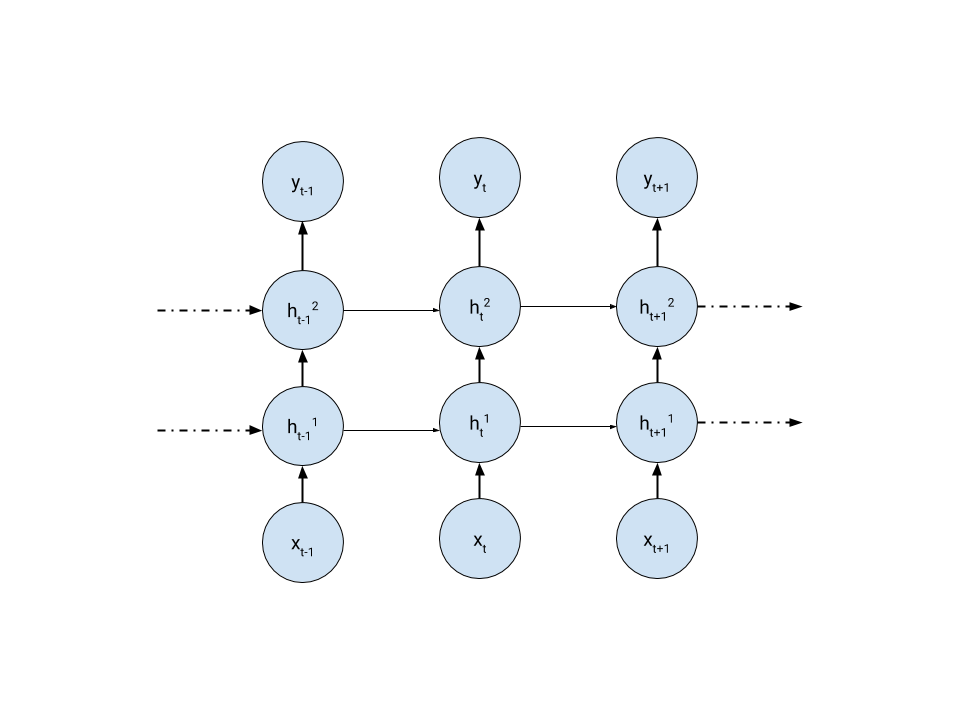
\includegraphics[scale=0.4]{rnn_diagram}
\caption{Stacked RNN.}
\label{fig:rnndiagram}
\end{figure}

%TODO: ADD REFERENCE TO ZAREMBA.
Let's start defining the equations for the LSTM cells. (Zaremba el al. 2014)
The memory cell $c_t$ contains the information of a unit. The gates controll how
much of that information should be memorized or forgotten to be sent to the next
step.
\begin{equation}
c^j_t = f^j_t c^j_{t-1} + i^j_t \widetilde{c}^j_t
\end{equation}
where
\begin{equation}
\widetilde{c}_t = \tanh{(W_c x_t + U_c h_{t-1})}
\end{equation}
Input $i_t$ and forget $f_t$ gates are calculated from previuos hidden states.
$h_{t-1}$
\begin{equation}
i_t = \sigma{(W_i x_t + U_i h_{t-1})}
\end{equation}
\begin{equation}
f_t = \sigma{(W_f x_t + U_f h_{t-1})}
\end{equation}
$\sigma{(.)}$ is an element-wise logistic sigmoid function. $x_t$ is the input
vector.

When we have the result of the memory content. The hidden state $h^j_t$ of the
$j$-th LSTM unit is calculated as:
\begin{equation}
h^j_t = o^j_t \tanh{(c^j_t)}
\end{equation}
The output gate $o_t$ controls how much memory is exposed:
\begin{equation}
o_t = \sigma{(W_o x_t + U_o h_{t-1})}
\end{equation}

LSTM cells help to memorize long term data dependencies.

The model's prediction $\hat{y}_t$ is obtained by:
\begin{equation}
\hat{y}_t = \textrm{softmax} (h^2_t)
\end{equation}
Notice that \textit{softmax} is is being applied only to the topmost hidden
layer on the stack.  In our rnn diagram (see figure~\ref{fig:rnndiagram}) $h^2_t
= y^t$

The evaluation of the model was done with a technical metric:
\textit{perplexity}, and by engagement metrics: \textit{users' replies} and
\textit{upvotes}. You can think of perplexity as a measure of how perplex or
surprised is the model of comparing the results it created with a validation
dataset. To obtain perplexity we must first calculate \textit{loss}. Loss allows
the model to determine how far away from the correct result is its
prediction, generally speaking the less the distance the better. The model
optimizes for minimizing this loss. Note that optimizing to much can cause
\textit{overfitting}, making our model incapable of generalize its guesses.

\begin{equation}
\textrm{loss} = -\frac{1}{N}\sum_{i=1}^{N} \ln{(\hat{y})}
\end{equation}

Then perplexity is defined as:

\begin{equation}
\textrm{perplexity} = e^{\textrm{loss}}
\end{equation}


\section{Experiment}
The dataset used in the experiment was 31 GB of an entire month's of reddit
comments. It has comment's metadata such as: score, subreddit, body and author.
I sectioned it to use a single subreddit (theme/topic). I decided to use the
``funny'' subreddit, which is one of the most popular subreddits. This subset
arrived to 450 MB of comments. Then to bias the model towards better quality
comments pre-evaluated by Reddit's community with the score field, I filtered
the comments to only keep the ones with score bigger than 10 (see
figure~\ref{fig:datasetsection}).  After this sectioning the dataset used for
training was about 13\% of the comments for the ``funny'' subreddit. Then I
generated a file to contain all of the comment's body, did a further separation
to create a train, test and validation datasets with 80\%, 10\% and 10\%
original body file size correspondingly.

\begin{figure}[h]
\centering
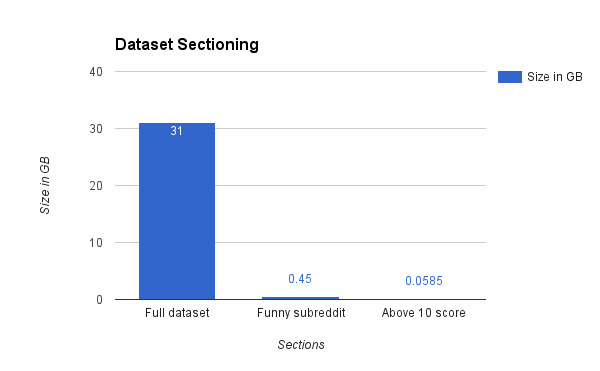
\includegraphics[scale=0.5]{dataset_sectioning}
\caption{Dataset sectioning.}
\label{fig:datasetsection}
\end{figure}

With the dataset ready I proceeded to train two models. One with LSTM and one
with GRU cells. This helped me compare the two models and choose the one that
performed the beter based solely on perplexity. I used two set of hyperparameter
configuration to train the models. You can see the hyperparameter sets used in
Table~\ref{table:hyperparameters}.

\begin{table}[h]
\caption{Used hyperparameter configurations for testing.}
\label{table:hyperparameters}
\centering
\begin{tabular}{lll}
\multicolumn{1}{c}{\bf Parameter}  &\multicolumn{1}{c}{\bf Small}
&\multicolumn{1}{c}{\bf Medium}
\\ \hline \\
batch\_size         &64         &64 \\
embed\_size         &50         &50 \\
hidden\_size        &100        &200 \\
num\_steps          &10         &20 \\
max\_epochs         &16         &26 \\
early\_stoping      &2          &2 \\
dropout             &0.5        &0.5 \\
learning\_rate      &0.001      &0.001 \\
num\_layers         &2          &2 \\
\end{tabular}
\end{table}

One of the main differences in both set of hyperparameters was the increase of
the hidden\_size parameter. By increasing it I arrived to better performance in
perplexity in both models. You can see the comparison of performance of both
models on figure~\ref{fig:perplexity}.

\begin{figure}[h]
\centering
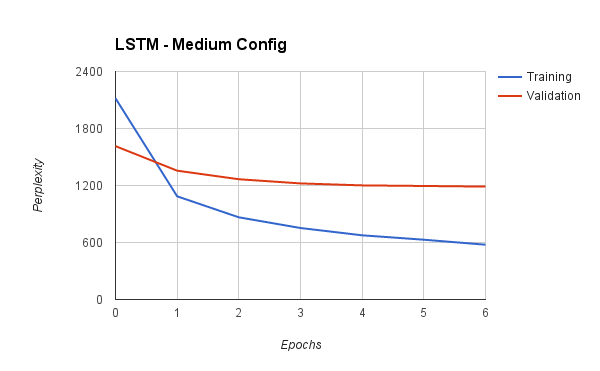
\includegraphics[scale=0.5]{lstm_medium_config}
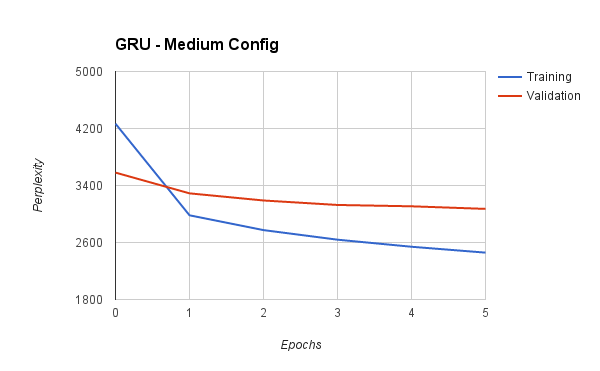
\includegraphics[scale=0.5]{gru_medium_config}
\caption{LSTM vs GRU models in training and validation perplexity.}
\label{fig:perplexity}
\end{figure}

We can clearly see that the model using LSTM cells was better than the one using
GRU cells at the given task with the same parameters. Given that conclusion I
decided to use the LSTM model's to generate test sentences.

To distribute the comments generated by my RNN I created a Reddit account called
Roy\_Nexus. I deliberatelly avoided to give any clear indication that this was
a bot, just to see people's reactions to it.

The bot worked as follows: It retrieved the top result of the feed ``rising''
under the subreddit ``funny''.  The decision to select this specific feed was
because it has posts that are not yet popular but have the potential to be at
the front page, by posting in here the bot had a chance of being relevant in the
case of selecting a future popular post. Once the bot had downloaded the
comment's information, it used the comment's title to give it as a seed of the
RNN's generative function. This way I provided some context to the RNN in hopes
of receiving back a sentence that was within the boundaries of the theme. Once
the RNN gave the output words, the bot uploaded them in a comment under the
previously selected post. Then the program slept for 15 minutes before repeating
the whole process again. The bot never commented twice on the same post.

The reaction obtained by the community was very clear: the comments generated by
the RNN were mostly non-sense or out of context. This resulted in a negative
response measured by the score the content received and by replies saying things
like ``are you having a stroke?'' or ``somebody has a case of Google translate
it seems''. You can see some screenshots of the generated comments on
figure~\ref{fig:comments}.
And you can see the some of the replies on figure~\ref{fig:replies}. Notice the
reply of the user that identified what I was doing to generate the sentences.

\begin{figure}[h]
\centering

\includegraphics[scale=0.5]{comment2}

\includegraphics[scale=0.5]{comment3}

\includegraphics[scale=0.5]{comment1}
\caption{Sample of the generated comments.}
\label{fig:comments}
\end{figure}

\begin{figure}[h]
\centering

\includegraphics[scale=0.5]{reply1}

\includegraphics[scale=0.5]{reply2}

\includegraphics[scale=0.5]{reply4}

\includegraphics[scale=0.5]{reply5}
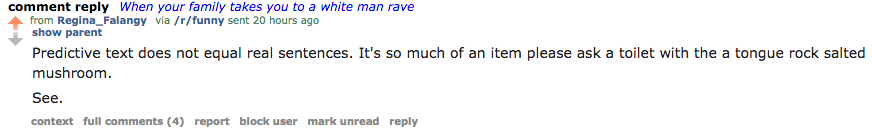
\includegraphics[scale=0.5]{reply3}
\caption{Sample of the replies by users.}
\label{fig:replies}
\end{figure}

After some days of publishing content on Reddit the the bot got tracked down and
banned from the subreddit ``funny'' by the moderators, giving end to the
experiment. On Table~\ref{table:engagement} you can see a summary of the number
of comments, replies and final comment score the bot got when finished the
experiment.

\begin{table}[t]
\caption{Engagement metrics.}
\label{table:engagement}
\begin{center}
\begin{tabular}{ll}
\multicolumn{1}{c}{\bf Concept}  &\multicolumn{1}{c}{\bf Value}
\\ \hline \\
Comments         &41 \\
Replies          &20 \\
Score            &-65 \\
\end{tabular}
\end{center}
\end{table}

\section{Conclusion}
After such a sudden forced end of my experiment. I concluded that the RNN didn't
have any sufficient consideration for the context of which it was being asked to
generate text. The title seed provided wasn't enough to guide the RNN to an
specific theme, much less to a set of themes. This task proved to be a very hard
problem.

I also think that the perplexity metric can be improved by first using more
data to train the model, second giving it more time to train and third
increasing the size of the hidden layer (as experiments concluded).

For furter extensions it would be illustrative to use a Gated Feedback RNN (GF-RNN),
this model had shown to be superior to the basic stacked RNN-LSTM, RNN-GRU
models in previous experiments and are promising. Is also interesting to mix
different models to aid in the problem of context and sentence understanding.
For example, integrating to a syntactic parser, that works by passing the input
sentences to tag each word with a part-of-speech (POS) tag that describes the
word's syntactic function, and determines the syntactic relationship between
words in the sentence, represented by a tree (see figure~\ref{fig:parsetree}).
This will help to understand the input and output sentence of the RNN.

\begin{figure}[h]
\centering
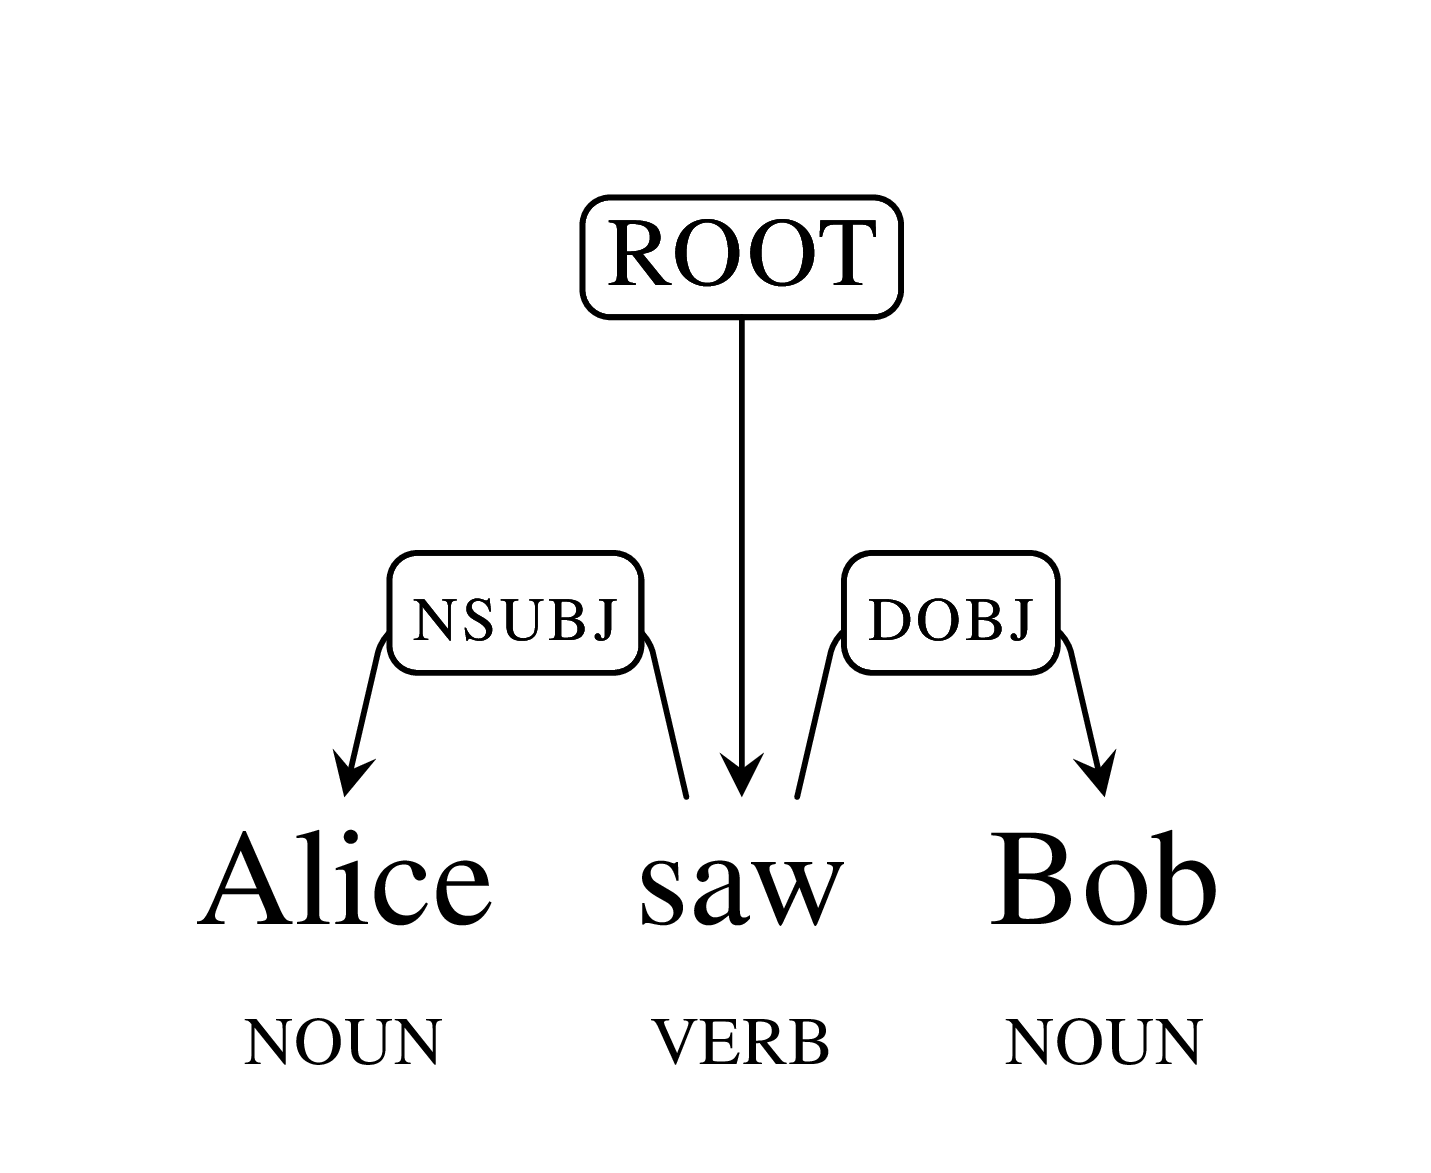
\includegraphics[scale=0.1]{parse_tree}
\caption{Parse tree of the phrase: ``Alice saw Bob''}
\label{fig:parsetree}
\end{figure}

\clearpage
\section{References}
Mikolov, Martin Karafiát, Lukás Burget, Jan Cernocký, Sanjeev Khudanpur:
Recurrent neural network based language model. INTERSPEECH 2010: 104\-1048

Sepp Hochreiter, J{\"u}rgen Schmidhuber: Long Short-Term Memory. 1997.

Zaremba, Wojciech and Sutskever, Ilya. Learning to execute.
arXiv preprint arXiv:1410.4615, 2014.

Junyoung Chung, Caglar Gulcehre, Kyunghyun Cho, Yoshua Bengio: Gated Feeback
Recurrent Neural Networks. arXiv:1502.02367. 2015

Reddit. \url{www.reddit.com}

Reddit dataset used \url{https://www.reddit.com/r/datasets/comments/3bxlg7/i_have_every_publicly_available_reddit_comment}

Announcing SyntaxNet: The World’s Most Accurate Parser Goes Open Source. \url{http://googleresearch.blogspot.com/2016/05/announcing-syntaxnet-worlds-most.html}
\end{document}
